\chapter{Primjer} \label{chapter:primjer}

U ovom poglavlju prikazan je primjer izrade jezerskog skladišta podataka i toka
podataka definiranog u poglavlju~(\ref{section:arhitektura_i_tok_podataka}). Za
ostvarivanje sloja obrade podataka korišten je Apache Spark
(poglavlje~(\ref{section:spark})), a za ostvarivanje sloja skladištenja podataka
korišten je Delta Lake (poglavlje~(\ref{section:delta_lake})). Za ostvarivanje
sloja unosa podata mogao se koristiti Apache Airflow, Azure Data Factory ili
neki slični alat. U ovom primjeru nije realiziran sloj unosa podataka jer bi
se sveo na kopiranje podataka iz jednog direktorija u drugi. U nastavku je
opisan postupak izrade jezerskog skladišta podataka i dimenzijskog modela
podataka.

\section{Opis zadatka} \label{section:opis_zadatka}

Izraditi jezersko skladište podataka i dimenzijski model podataka (vidjeti
\citep{dimensionalmodel2023}) za analizu iz podataka sa sljedećom strukturom:
\begin{description}
    \item[date] datum,
    \item[name] tekst,
    \item[phone] tekst,
    \item[email] tekst,
    \item[country] tekst,
    \item[colour] tekst,
    \item[currency] tekst.      
\end{description}
Dana struktura podataka je struktura sirovih podataka. Sirovi podaci su generirani
pomoću stranice \href{https://generatedata.com/}{\textit{generatedata.com}}. Sirovi
podaci su u formatu CSV i nalaze se u datoteci \texttt{sample\_data.csv} u
direktoriju \texttt{data} kako je prikazano na
slici~(\ref{figure:lakehouse_directory_structure}). Potrebno je izraditi
brončani, srebrni i zlatni sloj jezerskog skladišta podataka. U brončani sloj
treba učitati sirove podatke, kojima su dodana polja `batch\_date' i
`input\_file'. U srebrni sloj treba učitati podatke iz brončanog sloja i
kreirati dimenzijske tablice `colour', `country' i `person' i činjeničnu
tablicu `fact\_table'. U zlatni sloj treba učitati podatke iz srebrnog sloja i
kreirati činjenične tablice `most\_bought\_colour\_per\_month', `person\_spent'
i `spent\_per\_day'. Također, za tablice `spent\_per\_day' treba napraviti i
vizualizaciju podataka. Konačno jezersko skladište podataka bi trebalo imati
strukturu direktorija i datoteka prikazano na
slici~(\ref{figure:lakehouse_directory_structure}). U nastavku je opisan
postupak izrade jezerskog skladišta podataka i dimenzijskog modela podataka.

\begin{figure}
    \centering
    \footnotesize
    \begin{forest}
        for tree={
        font=\ttfamily,
        grow'=0,
        child anchor=west,
        parent anchor=south,
        anchor=west,
        calign=first,
        edge path={
            \noexpand\path [draw, \forestoption{edge}]
            (!u.south west) +(7.5pt,0) |- node[fill,inner sep=1.25pt] {} (.child anchor)\forestoption{edge label};
        },
        before typesetting nodes={
            if n=1
            {insert before={[,phantom]}}
            {}
        },
        fit=band,
        before computing xy={l=15pt},
        }
    [root
        [data
            [sample\_data.csv]
        ]
        [lakehouse
            [bronze
                [bronze\_data]
            ]
            [silver
                [colour]
                [country]
                [person]
                [fact\_table]
            ]
            [gold
                [most\_bought\_colour\_per\_month]
                [person\_spent]
                [spent\_per\_day]
            ]
        ]
    ]
    \end{forest}
    \caption{Struktura direktorija i datoteka u primjeru jednostavnog jezerskog skladišta podataka.}
    \label{figure:lakehouse_directory_structure}
\end{figure}

\section{Unos podataka u brončani sloj} \label{section:unos_podataka_u_broncani_sloj}

Programski kod~(\ref{lst:bronze_data}) prikazuje dio skripte koja gradi tablicu
`bronze\_data' u jezerskom skladištu podataka. Za čitanje sirovih podataka
koristi se funkcija \texttt{read\_raw\_data} koja koristi Sparkov DataFrameReader 
klasu za čitanje podataka iz datoteke \texttt{sample\_data.csv}. Nakon čitanja
sirovih podataka dodaju se polja `batch\_date' i `input\_file' koja se koriste za
praćenje podataka kroz jezersko skladište podataka. Polje `batch\_date' sadrži
datum kada su podaci učitani u jezersko skladište podataka, a polje
`input\_file' sadrži naziv datoteke iz koje su podaci učitani. Nakon dodavanja
polja podaci se zapisuju u jezersko skladište podataka u tablicu `bronze\_data'.

\begin{lstlisting}[
    language=Python, 
    caption={Dio skripte koja gradi tablicu `bronze\_data' u jezerskom skladištu podataka \citep{simplelakehouse2023}.}, 
    label={lst:bronze_data},
    basicstyle=\footnotesize
]
raw_df = read_raw_data(
    path="data/sample_data.csv",
    schema=schema,
    spark=spark
)

# Add batch date and input file name to raw data
batch_date = datetime.now().strftime("%Y-%m-%d")
raw_df = raw_df.withColumn(
    "batch_date",
    to_date(
        lit(batch_date),
        "yyyy-MM-dd"
    )
)
raw_df = raw_df.withColumn(
    "input_file",
    input_file_name()
)

# Write raw data to lakehouse bronze layer
write_to_lakehouse(
    df=raw_df,
    path="lakehouse/bronze/bronze_data",
    partition=True
)
\end{lstlisting}

\section{Unos podataka u srebrni sloj} \label{section:unos_podataka_u_srebrni_sloj}

Kod unosa podataka u srebrni sloj potrebno je napraviti dimenzijske tablice i 
činjeničnu tablicu. Programski kod~(\ref{lst:fact_table}) prikazuje dio
skripte koja gradi tablicu `fact\_table' u jezerskom skladištu podataka. Za
izradu tablice `fact\_table' potrebno je učitati podatke iz tablice
`bronze\_data' i kreirati dimenzijske tablice `person', `country' i `colour'. 
Dimenzijske tablice se grade tako da se iz tablice `bronze\_data' izvuku
potrebni stupci i uklone duplikati. Nakon toga se dimenzijskim tablicama dodaju
surogatni ključevi. Surogatni ključevi se dodaju tako da se dimenzijske tablice
mogu spajati s činjeničnom tablicom samo preko jednog stupca. Nakon dodavanja
surogatnih ključeva dimenzijske tablice se spajaju s tablicom `bronze\_data'. 
Iz tablice dobivene spajanjem se odabiru samo potrebni stupci. Potrebni stupci
su surogatni ključevi dimenzijskih tablica, datumski stupci i mjere. Nakon
odabira stupaca tablica se zapisuje u jezersko skladište podataka u tablicu
`fact\_table'. Opisani postupak za kreiranje činjenične tablice izradi je u
programskom kodu~(\ref{lst:fact_table}). 

\begin{lstlisting}[
    language=Python, 
    caption={Dio skripte koja stvara tablicu `fact\_table' u jezerskom skladištu podataka \citep{simplelakehouse2023}.}, 
    label={lst:fact_table},
    basicstyle=\footnotesize
]
fact_df = bronze_df.join(
    person_df,
    [
        df.first_name == person_df.first_name,
        df.last_name == person_df.last_name,
        df.phone == person_df.phone,
        df.email == person_df.email,
        df.country == person_df.country
    ],
    how='inner'
)

fact_df = fact_df.join(
    country_df,
    'country',
    how='inner'
)

fact_df = fact_df.join(
    colour_df,
    'colour',
    how='inner'
)

fact_df = fact_df.select(
    'date',
    'person_id',
    'country_id',
    'colour_id',
    'currency'
)

write_to_lakehouse(
    df=fact_df,
    path="lakehouse/silver/fact_table"
)
\end{lstlisting}

\section{Unos podataka u zlatni sloj} \label{section:unos_podataka_u_zlatni_sloj}

Kod unosa podataka u zlatni sloj potrebno je napraviti tablice
`most\_bought\_colour\_per\_month', `person\_spent' i `spent\_per\_day'.
Programski kod~(\ref{lst:spent_per_day}) prikazuje dio skripte koja gradi
tablicu `spent\_per\_day' u jezerskom skladištu podataka. Za izradu tablice
`spent\_per\_day' potrebno je učitati podatke iz tablice `fact\_table' i
izračunati ukupan iznos potrošen po danu. Nakon izračuna ukupnog iznosa
potrošenog po danu tablica se zapisuje u jezersko skladište podataka u tablicu
`spent\_per\_day'. Za tablice `most\_bought\_colour\_per\_month' i
`person\_spent' postupak je sličan kao i za tablicu `spent\_per\_day'. Postupak
se ralikuje po načinu računanju mjera i potrebnih dodatnih dimenzijskih tablica.
Na slici~(\ref{figure:spent_per_day_graph}) se vidi graf koji prikazuje podatke
iz tablice `spent\_per\_day'. Na grafu se prikazuje zadnjih deset dana. Na
x-osi se nalazi datum, a na y-osi se nalazi ukupan iznos potrošen po danu.

\begin{lstlisting}[
    language=Python, 
    caption={Dio skripte koja gradi tablicu `spent\_per\_day' u jezerskom skladištu podataka \citep{simplelakehouse2023}.}, 
    label={lst:spent_per_day},
    basicstyle=\footnotesize
]
spent_per_day_df = (
    fact_df
    .groupBy('date')
    .sum('currency')
    .withColumnRenamed(
        'sum(currency)', 
        'spent_per_day'
    )
)

write_to_lakehouse(
    df=spent_per_day_df,
    path="lakehouse/gold/spent_per_day"
)
\end{lstlisting}

\begin{figure}
    \centering
    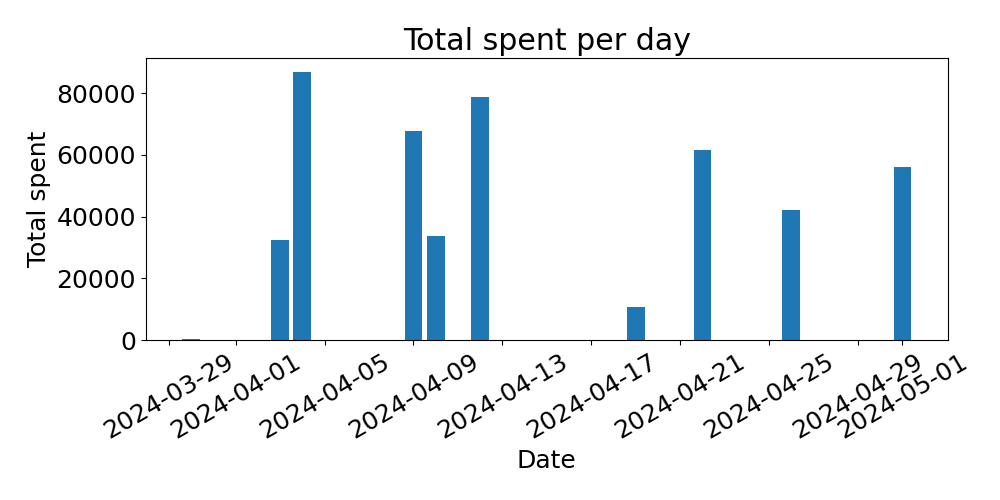
\includegraphics[width=0.8\linewidth]{images/myplot.png}
    \caption{Graf koji prikazuje podatke iz tablice `spent\_per\_day'.}
    \label{figure:spent_per_day_graph}
\end{figure}